
\chapter{Results and Discussion}

\label{Chapter5} % For referencing the chapter elsewhere, use \ref{Chapter1} 

\section{Results}

To test the AI's performance, we set up the following experiment. First, the subject was given time to familiarize and acclimate themselves to the controls and dynamics of the game. Afterwards, the subject played a series of 20 second long matches against a computer opponent that follows a set defensive behavior pattern. A random match from this pool was selected to be the demonstration session, while the rest were grouped into a set of holdout sessions. We then used the data from the demonstration session to create 3 kinds of agents. One of the agents used our novel search technique. The other agents implemented N-grams and the adaptive GhostAI and served as a point of comparison. We then recorded several sessions where each of these agents was pitted against the same computer opponent that the subject faced.

The recorded sessions were then evaluated along 3 criteria, Similarity, Effectivenss, and Qualitative Judgement.

\subsection{Similarity}

To measure similarity, we used a metric based on the work by \cite{simil}. Given event sequences $A$ and $B$, let $H_A$ and $H_B$ represent the underlying histogram of all $n$-Grams where $1 \le n \le 3$. Then let $S_A$ and $S_B$ be the number of unique substrings in $H_A$ and $H_B$ respectively, and let $f(s|H)$ be the number of times substring $s$ appears in histogram $H$. The similarity metric is then defined as follows:

$$PlayerSim(A,B) = \sum_{s \in S_A \cup S_B} \frac{|f(s|H_A) - f(s|H_B)|}{f(s|H_A) + f(s|H_B)}$$

For our use case, we took the average similarity between the training session and the sessions recorded in each category.

\begin{table}[h]
	\centering
	\caption{ Similarity Measurements }
	\begin{tabular}	{| c | c | c | c | c | c |}
		\hline
		 & Holdout Session & ngram & GhostAI & Search AI & Unrelated player\\
		\hline
		Mean &
		0.313 & 
		0.242 &
		0.197 &
		0.227 &
		0.307 		\\
		\hline
		Standard Deviation & 
		0.025 & 
		0.039 &
		0.019 &
		0.022 &
		0.070 		\\
		\hline
	\end{tabular}
	\label{Similarity}
\end{table}


\subsection{Effectiveness}
To measure Effectiveness, we compared the number of hits that were landed in the training session to the average number of hits recorded for each other category.

\begin{table}[h]
	\centering
	\caption{Effectiveness Measurements}
	\begin{tabular}	{| c | c | c | c | c | }
		\hline
		& Other Replay & ngram & GhostAI & Search AI \\
		\hline
		Mean &
		33.6 &
		29.6 &
		13.2 &
		15.8\\
		\hline
		Standard Deviation &
		6.6211781429 &
		18.3804243694 &
		2.92574776767 &
		4.95580467735 \\
		\hline
	\end{tabular}
	\label{Effectiveness}
\end{table}


\subsection{Qualitative Analysis}
For our qualitative analysis we also visually inspected heatmaps of the demonstrations like follows.

\begin{figure}[h]
	\centering
	\begin{subfigure}[h]{0.3\textwidth}
		\centering
		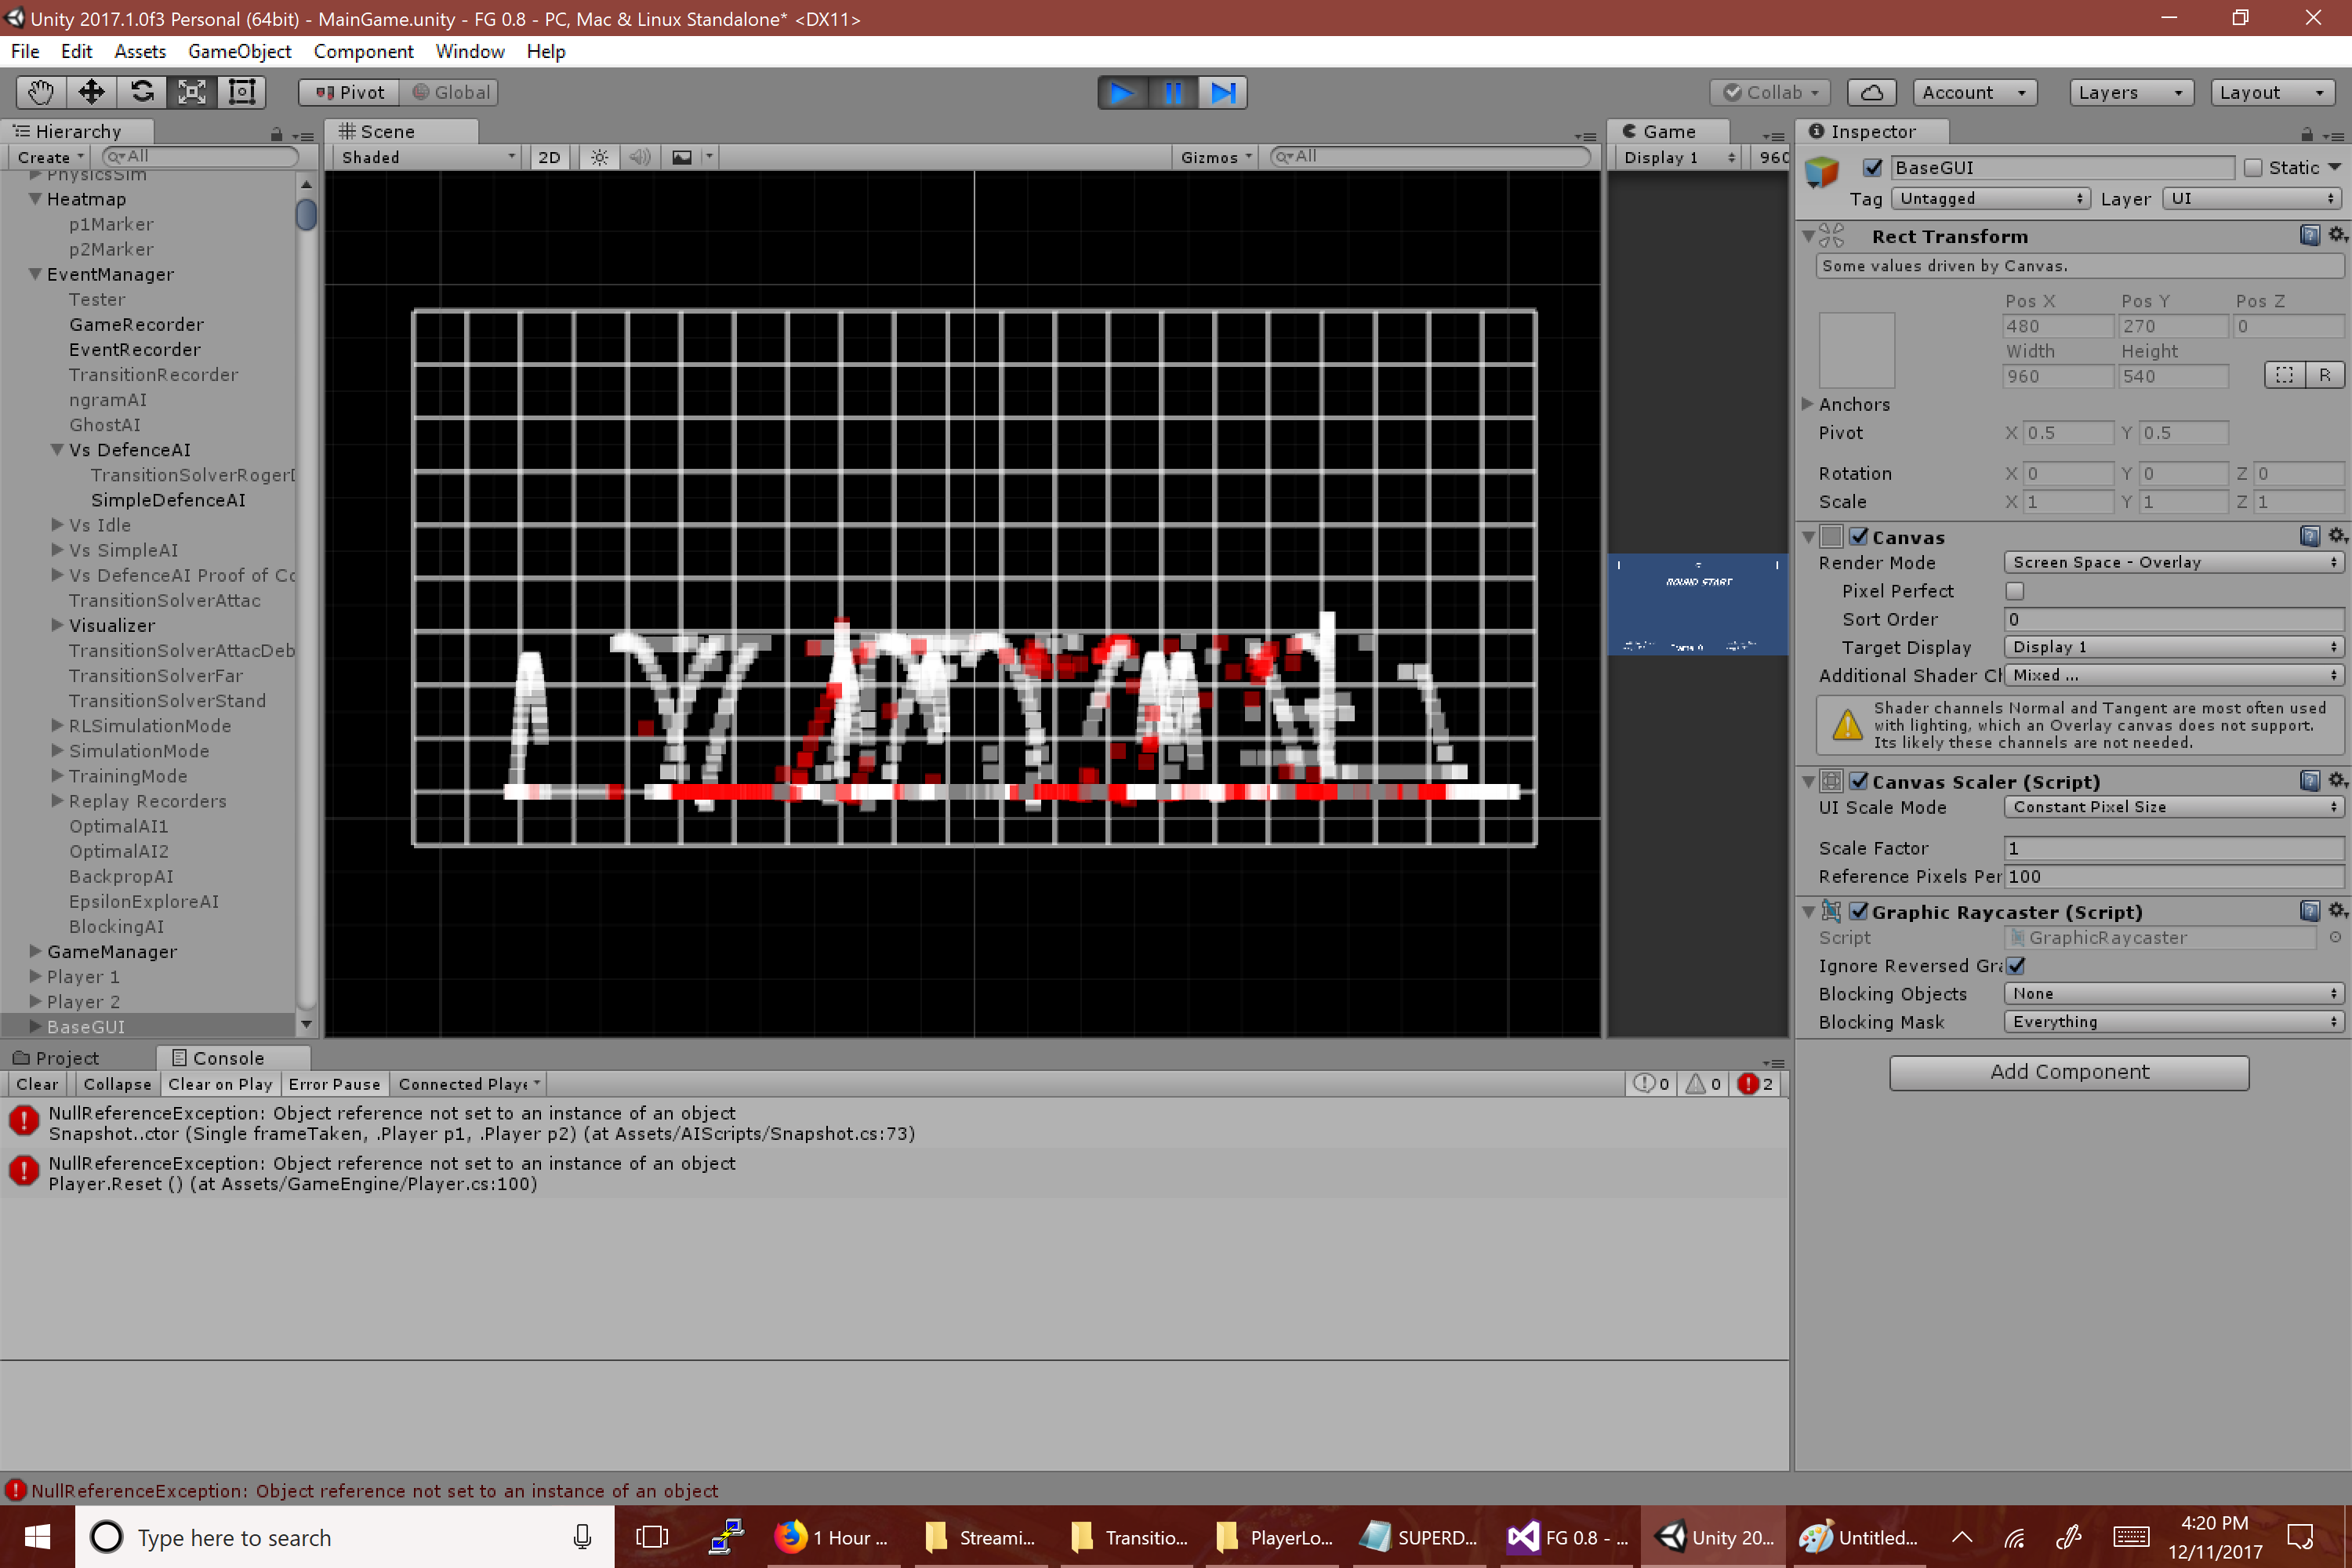
\includegraphics[width=\textwidth]{Figures/HeatmapOrig.png}
		\caption{case 1}
		\label{}
	\end{subfigure}
	\begin{subfigure}[h]{0.3\textwidth}
		\centering
		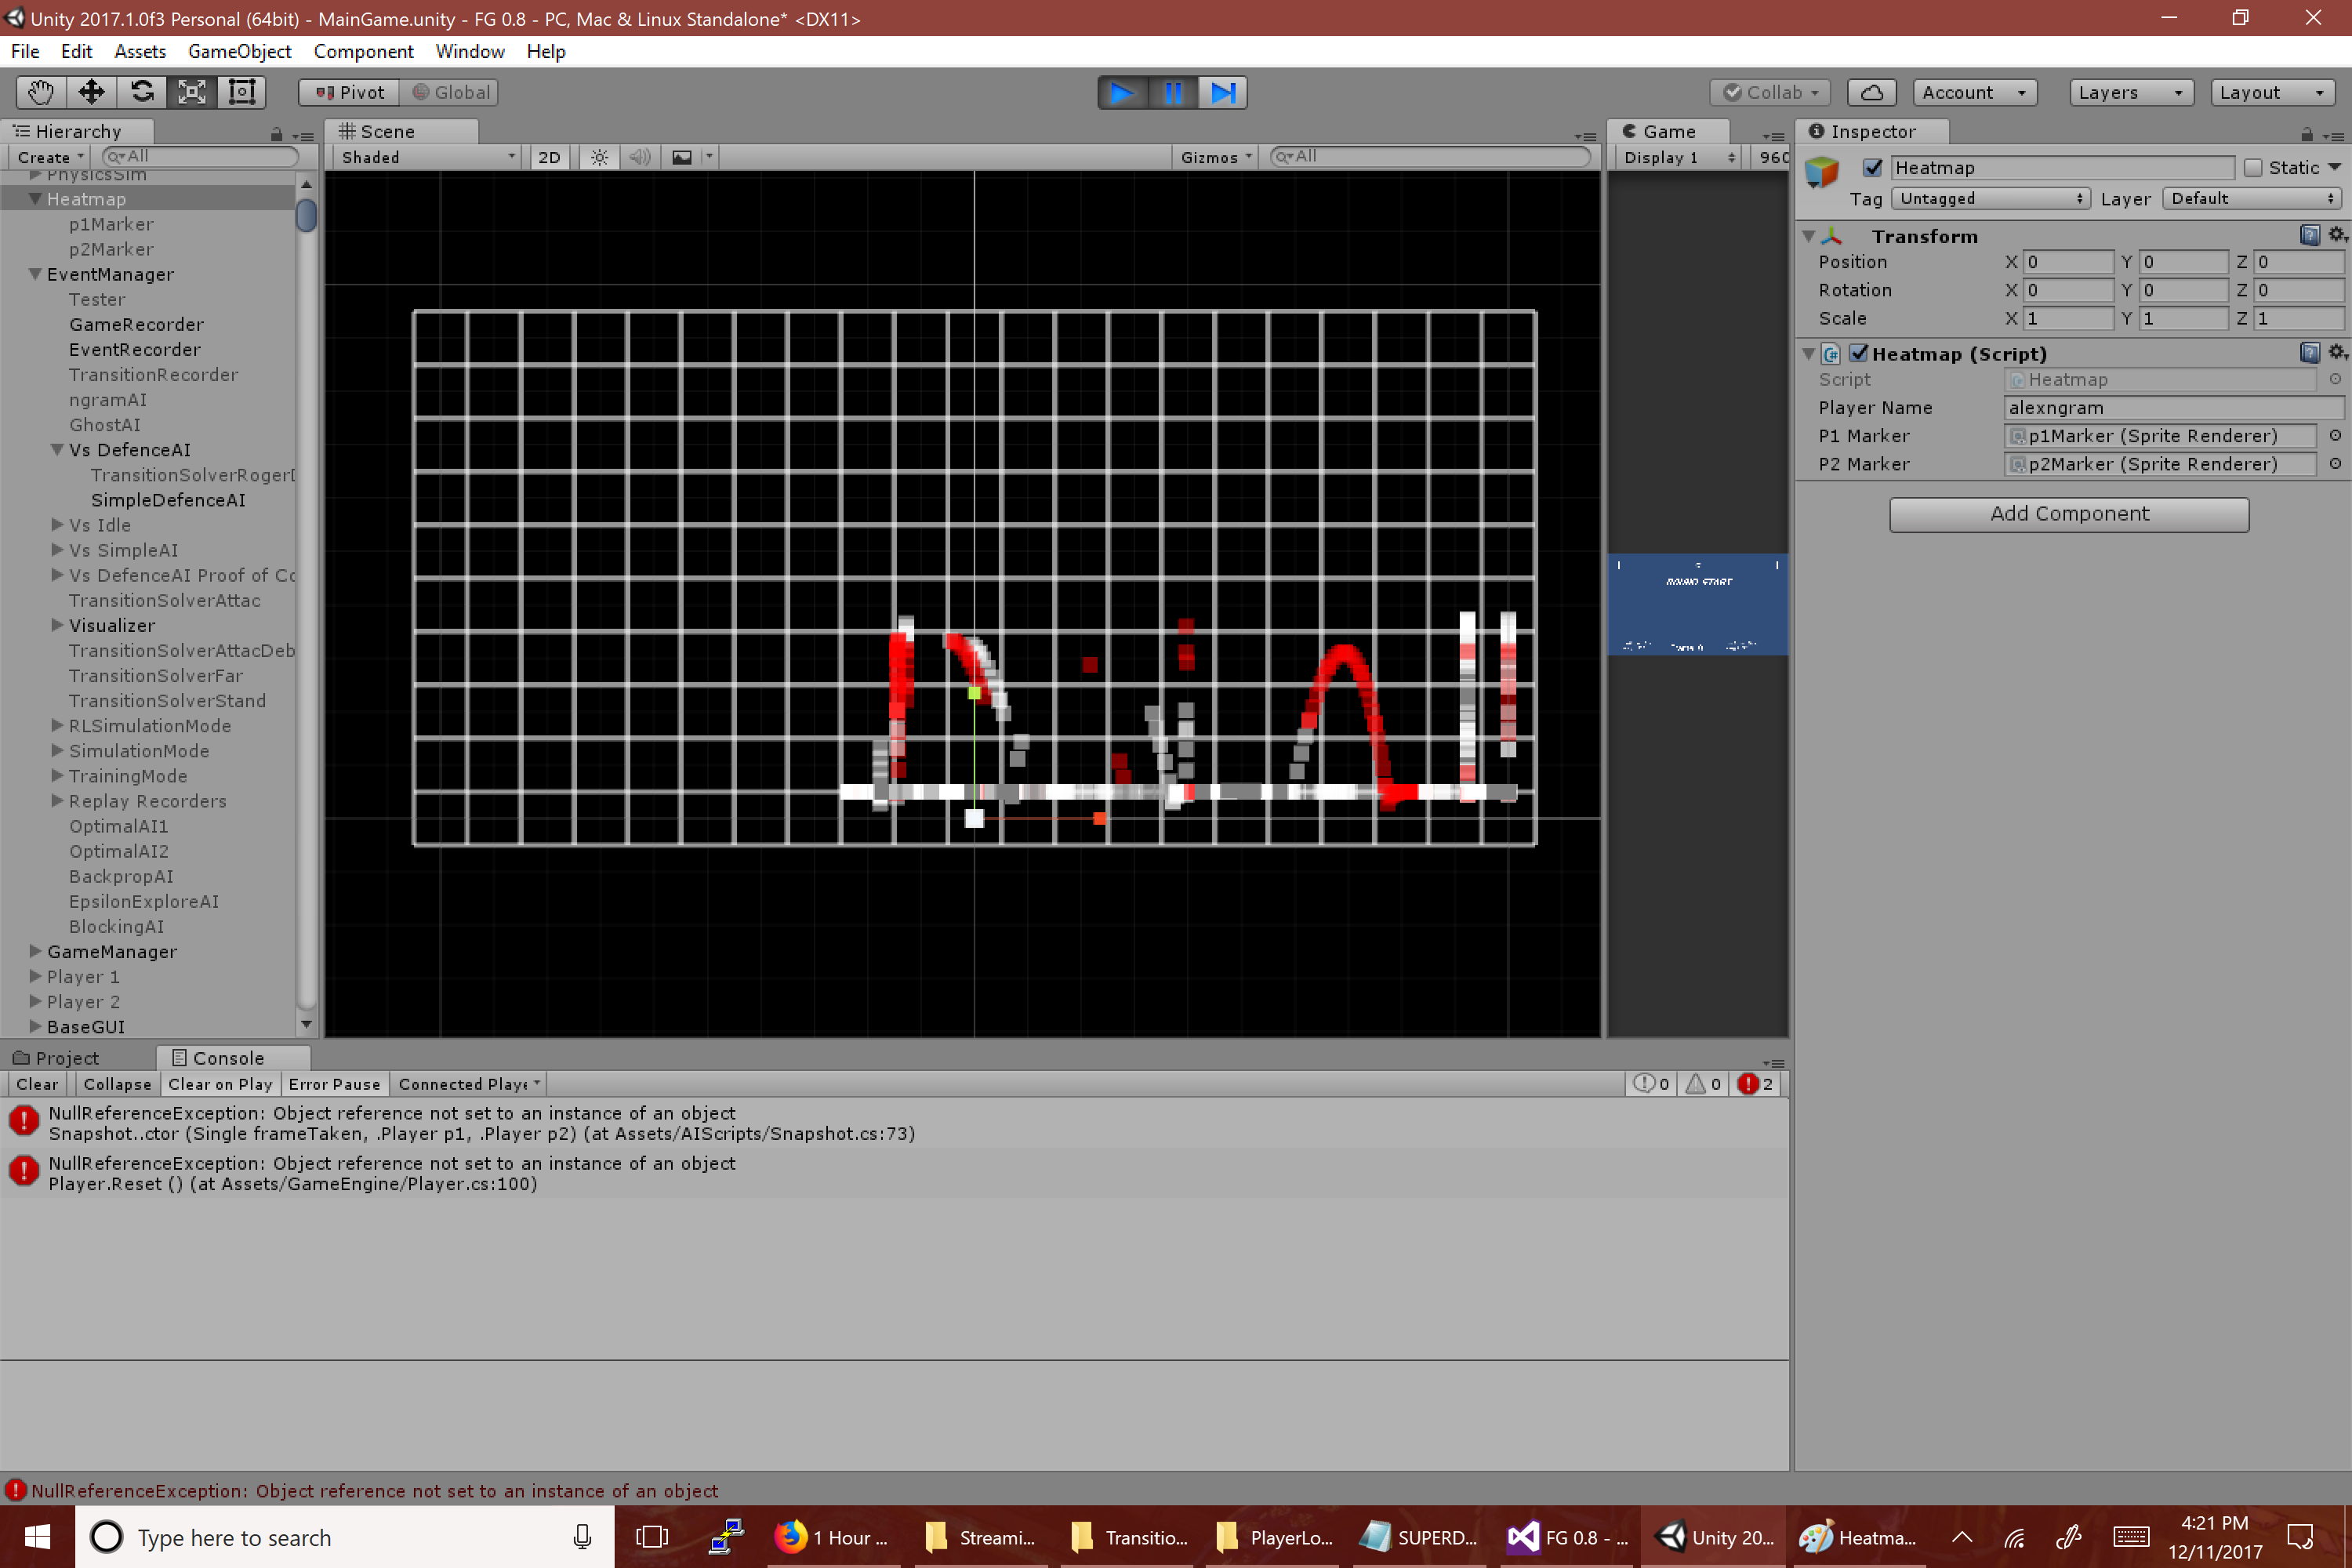
\includegraphics[width=\textwidth]{Figures/HeatmapNgram.png}
		\caption{case 2}
		\label{}
	\end{subfigure}
	\begin{subfigure}[h]{0.3\textwidth}
		\centering
		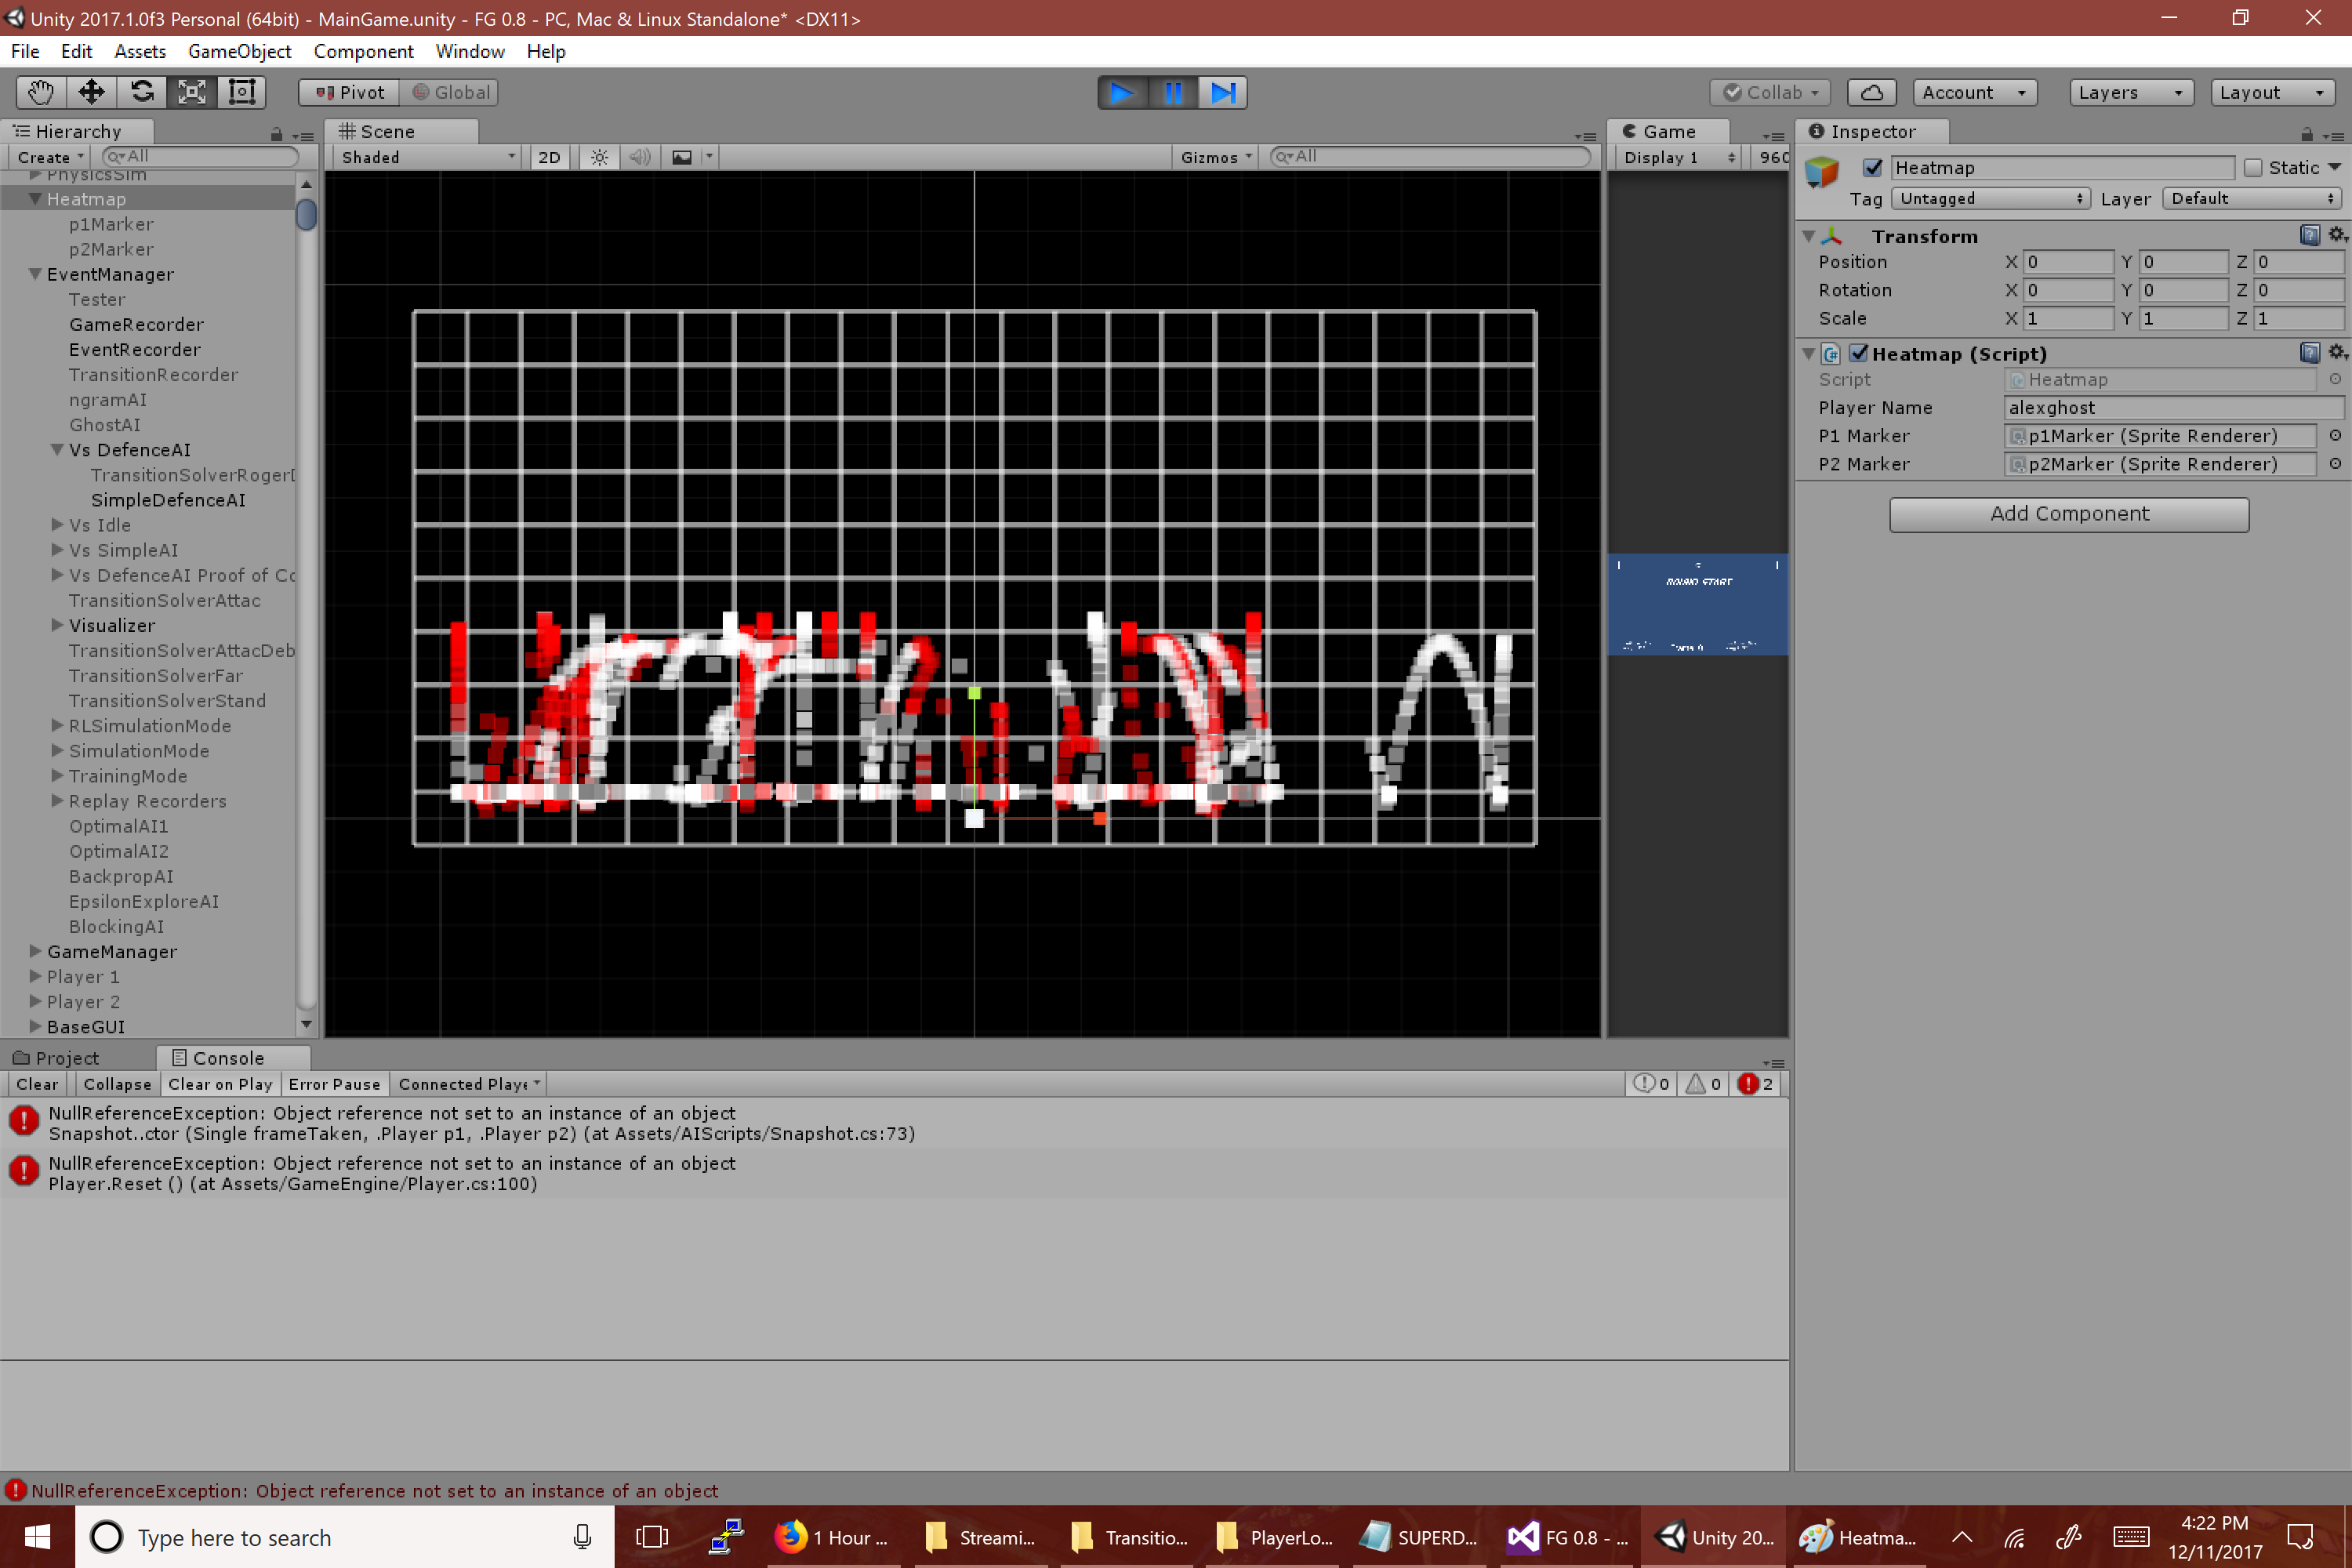
\includegraphics[width=\textwidth]{Figures/HeatmapGhost.png}
		\caption{case 3}
		\label{}
	\end{subfigure}
	\begin{subfigure}[h]{0.3\textwidth}
		\centering
		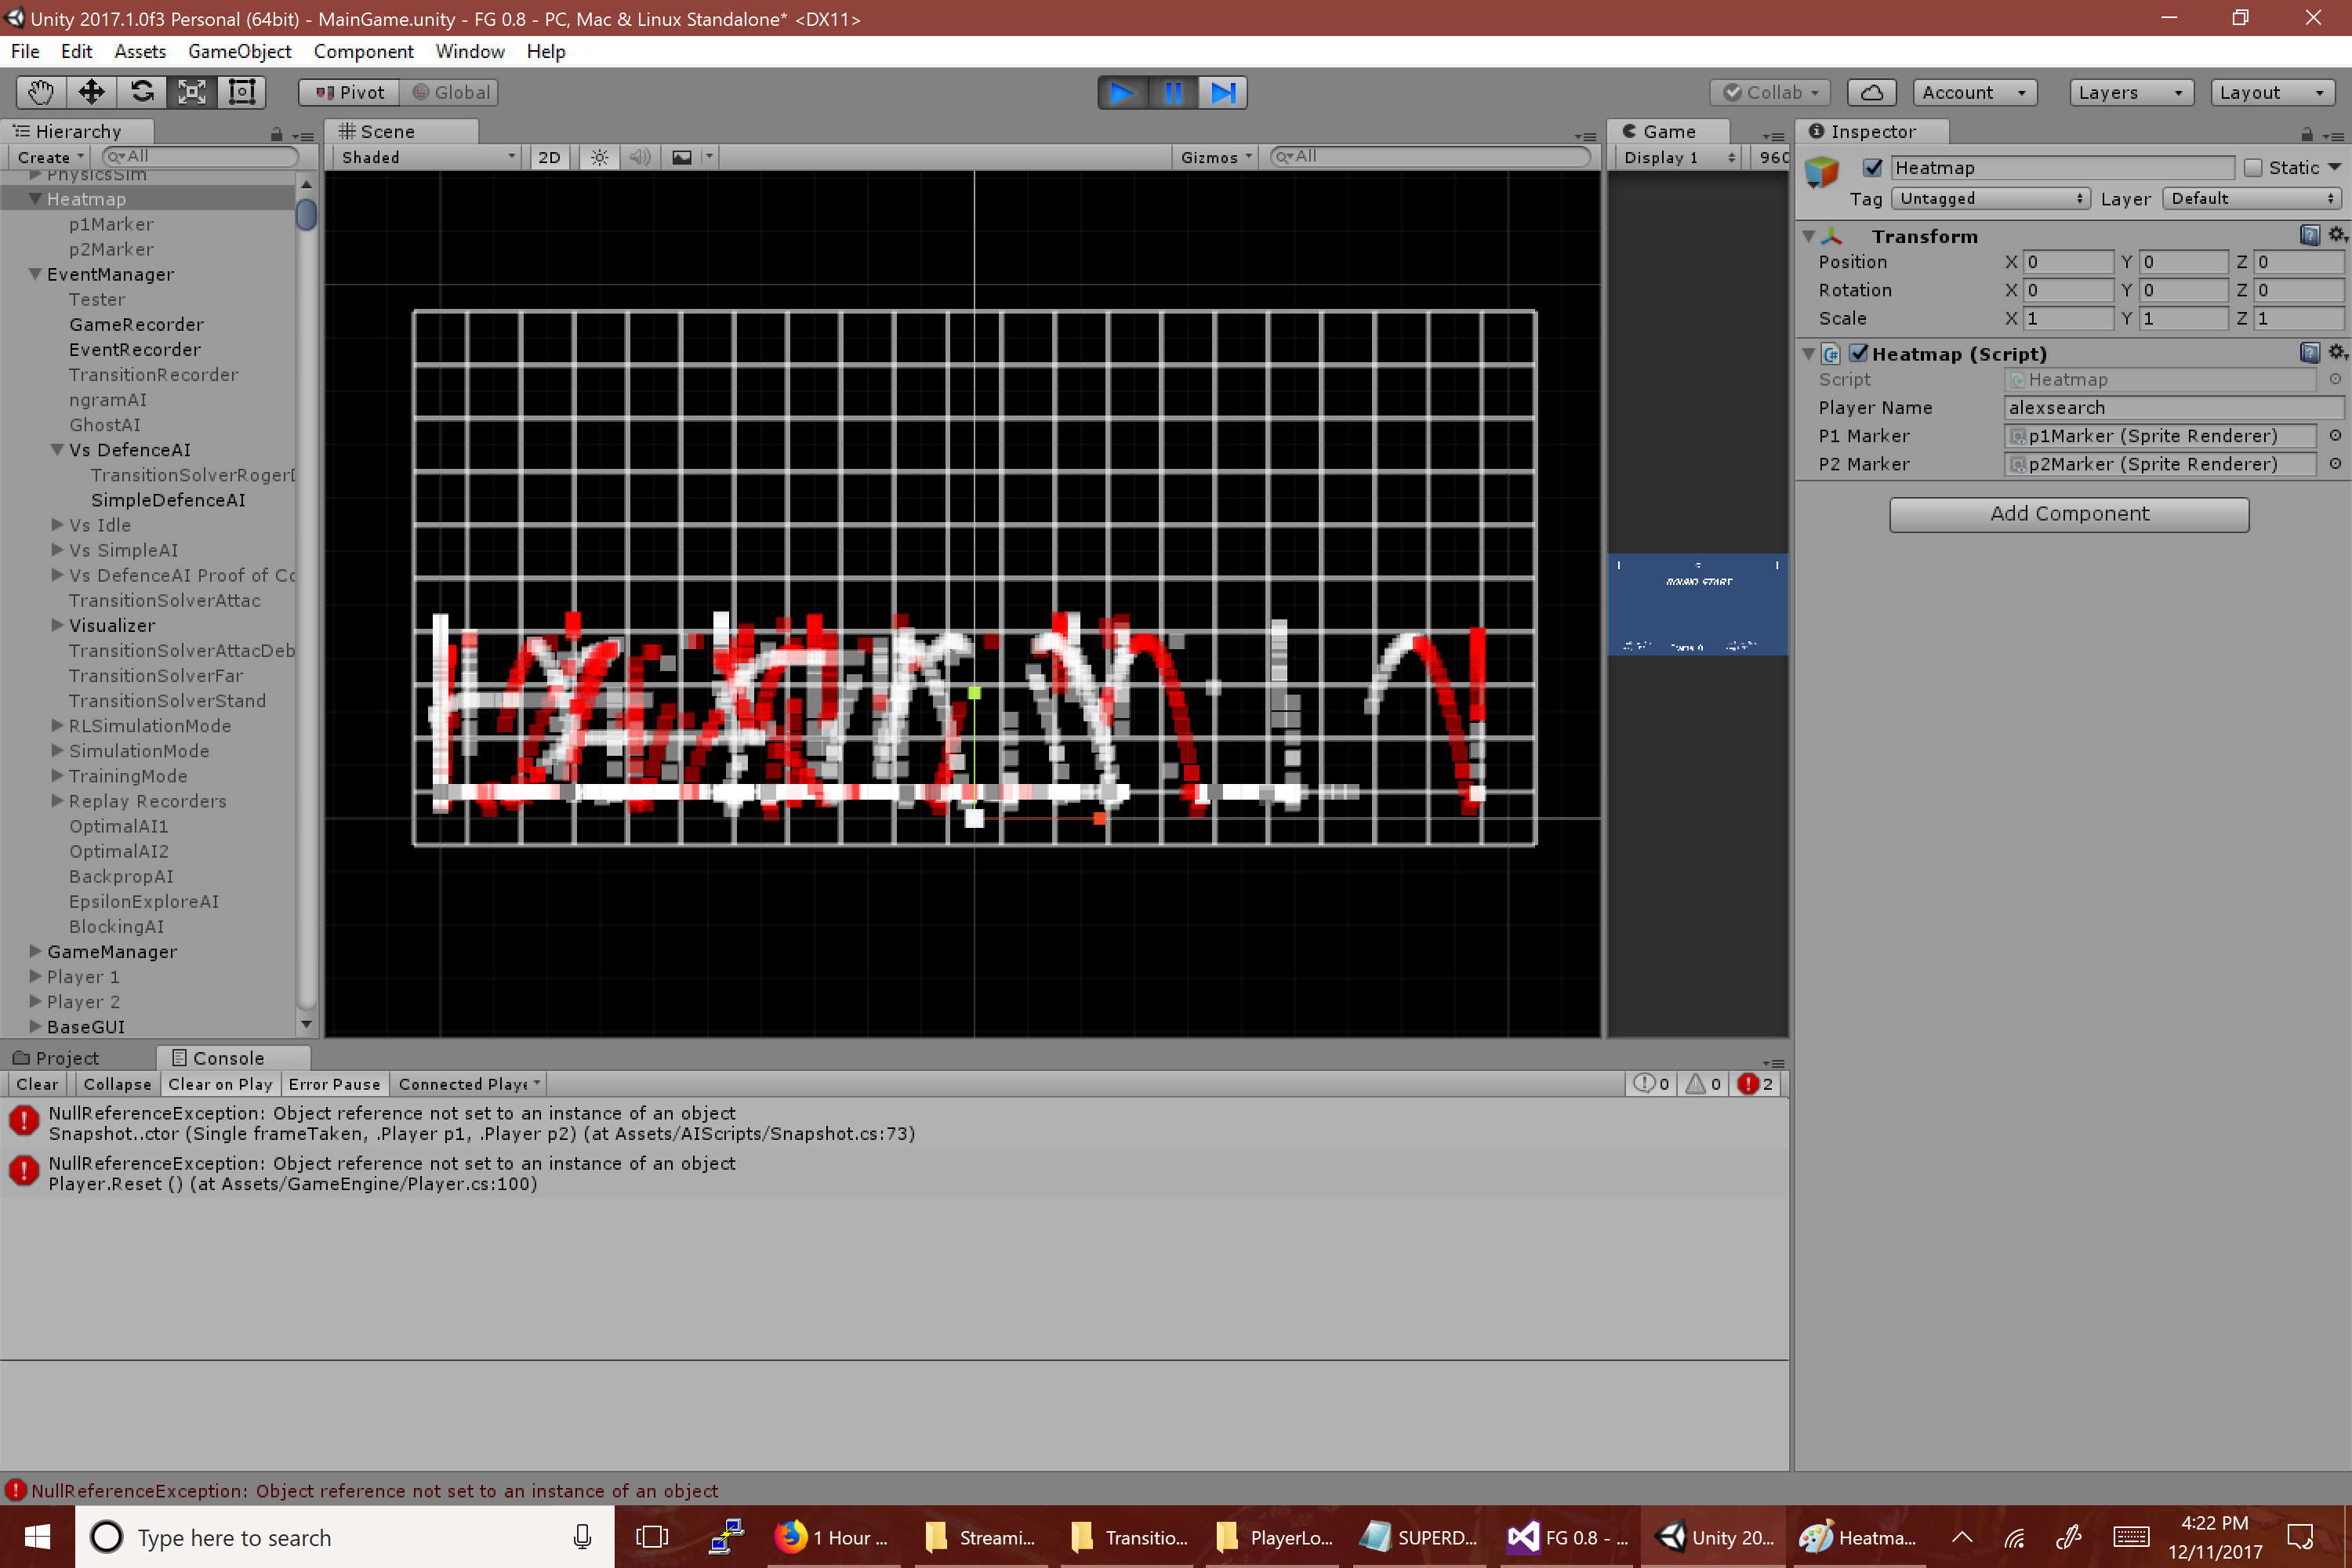
\includegraphics[width=\textwidth]{Figures/HeatmapAI.png}
		\caption{case 4}
		\label{}
	\end{subfigure}
	\begin{subfigure}[h]{0.3\textwidth}
		\centering
		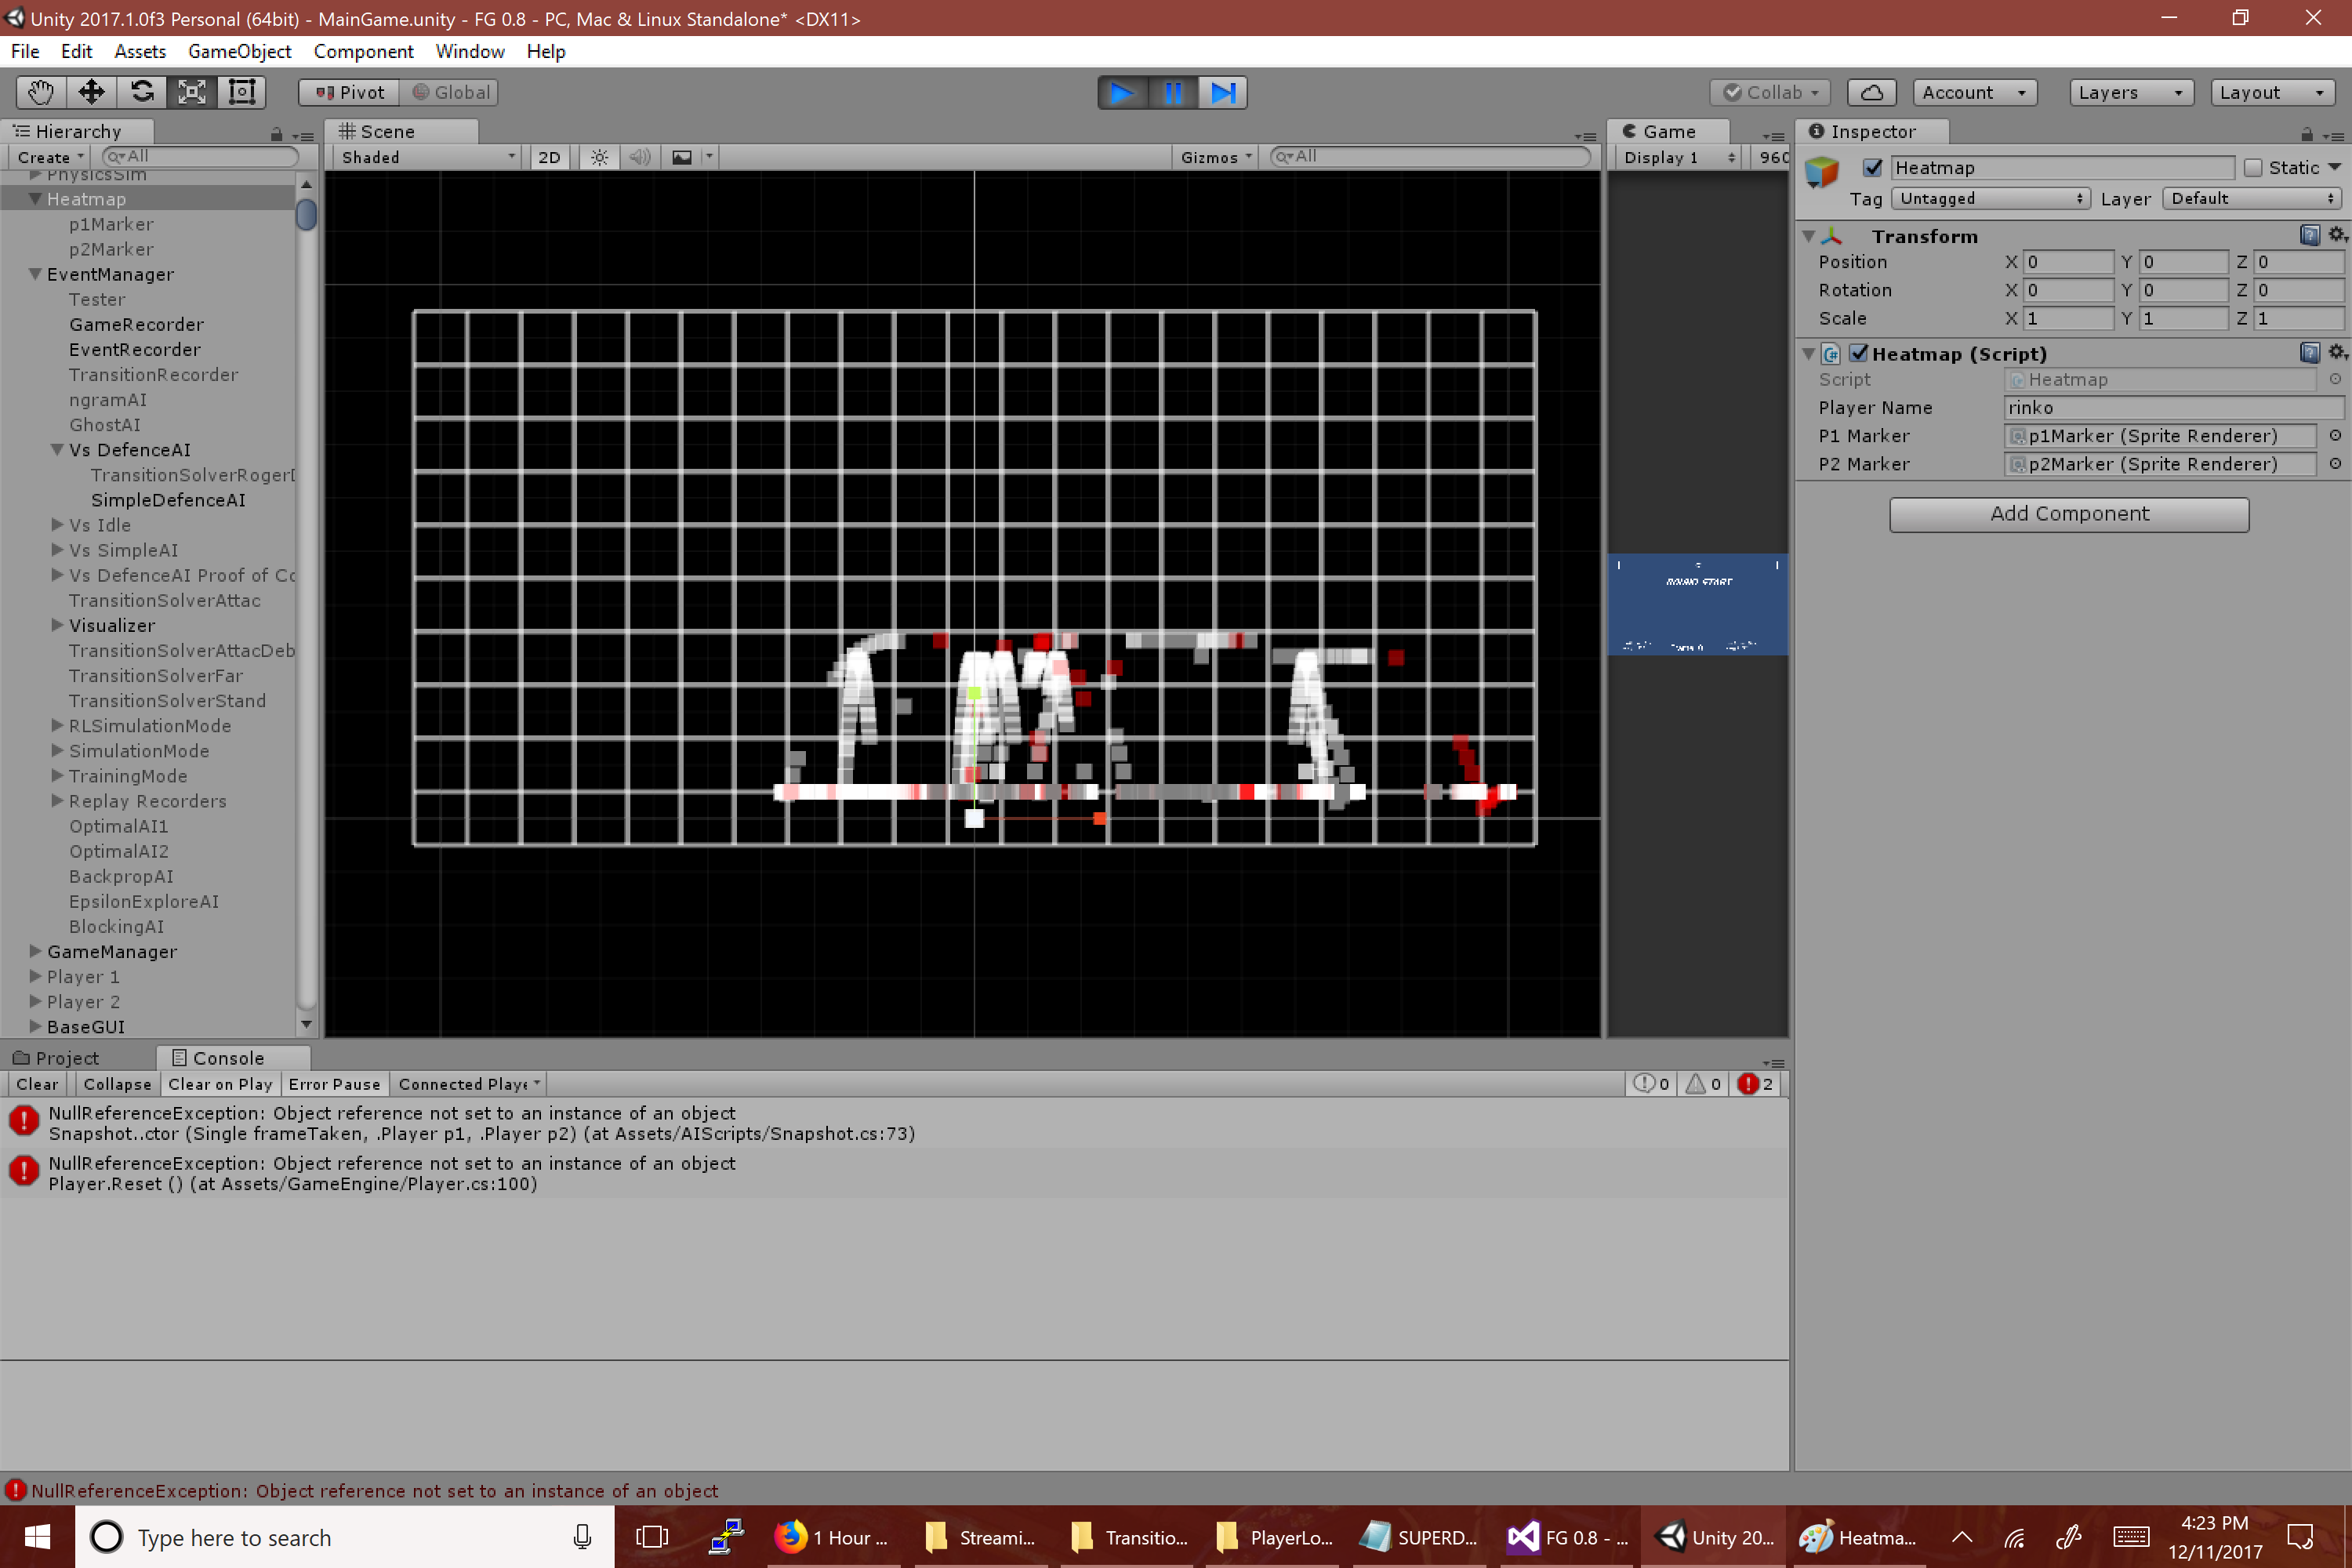
\includegraphics[width=\textwidth]{Figures/HeatmapOther.png}
		\caption{case 5}
		\label{}
	\end{subfigure}
\end{figure}


\section{Discussion}

From a qualitative standpoint, the Search AI's movement is the most natural. This is because plannning allows it to take broad motions before deciding to take a different action. However, both the Ghost AI and Search AI are prone to getting stuck into certain repeated patterns, a trait which to most people signifies a non-human player. This is likely because both GhostAI and Search AI try to reach the goal of hitting the opponent in an efficient manner. This adherence to an "optimal" kind of play can result in situations where the agent behaves greedily to a fault and comes off as non-human-like.

From an effectiveness point of view, it is difficult to judge. Though the ngram scored the highest, it's standard deviation is extremely high, which suggests that it may have scored well in some situations due to random chance. On the other hand, Search AI consistently scores higher than Ghost AI. This is likely because Ghost AI has to take time to adjust it's weights for taking the correct action, whereas Search AI innately has an understanding of the cause and effect of actions.

Lastly from a similarity point of view we perform about as expected, because of the nature of the similarity scoring function, the N-gram behaves in a way that naturally boosts that score. It is good to see however that Search AI doesn't lag too far behind, as it shows that it is better at maintaining the characteristic actions of the original player while still trying to reach a desired destination.